\title{Emojis and Weather}
\author{
        Darryl Hannan \\
                Villanova University
\and
	Emma Chin \\
		Villanova University
\and
	Matt Mador \\
		Villanova University
}
\date{\today}

\documentclass[12pt]{article}
\usepackage{graphicx}
\graphicspath{{images/}}

\begin{document}
\maketitle

\begin{abstract}
A significant amount of research has been done analyzing the impact weather has on emotional states. Most of these studies are survey based, and therefore have a small sample size. Here, we seek to overcome this problem through the use of social media. We analyze tweets from various geographic locations, extracting emojis. We use the distribution of emojis to represent the emotional state of a population. We use these representations to train a machine learning classifier that predicts the weather. Our model is approximately 88\% accurate, providing support for the link between weather and mood.
\end{abstract}

\section{Introduction}
The impact that weather has on mood is well established. Spasova (2011) found that abrupt transitions to unfavorable weather conditions has a negative effect on emotion.\cite{Spasova2011} Keller et al. (2005) found that time spent in pleasant weather results in better mood and improved memory.\cite{Keller2005} Some effects are more serious; seasonal effective disorder occurs occurs during winter months, when the days are shortest, and can result in serious cases depression.\cite{Melrose2015}

The effect that weather has on emotions varies significantly among individuals.\cite{Spasova2011} Therefore, large sample sizes are needed to discover correlations between specific weather patterns and emotional states. Traditionally, the only way to study this set of phenomena was through survey based methods, resulting in small sample sizes. We attempt to overcome this problem through the use of Twitter. By analyzing the emotions expressed in tweets for a given geographic location, we obtain an approximation of the collective emotional state of the population. This method also makes it significantly less expensive to collect data. By running the collection program on a server, we can continuously collect data indefinitely.

\section{Related Work}
Park et al. (2013) also utilize Twitter to gather emotional data.\cite{Park2013} They use a linear regression model to predict various variables such as temperature, humidity, and precipitation. Our approach differs in that Park et al. perform sentiment analysis on the tweets, whereas we use emojis to represent sentiment. By using emojis, we require significantly less preprocessing and impose less structure on the emotional representation that the model ultimately learns.

Baylis et al. (2017) use both Twitter and Facebook to collect emotional data. Using more than 3.5 billion social media posts in their model.\cite{Baylis2017} Their weather variable, referred to as cloud cover, is similar to the variable that we predict in our model. The primary difference in our model again lies in the use of emojis.

\section{Data}

\subsection{Emotion Data}
We collect tweets from 21 cities using Twitter's Streaming API via Tweepy\footnote{http://www.tweepy.org/}, targeting locations with high populations in order to maximize the number of data points. We preselected a list of 75 emojis that commonly represent various emotional states (Figure \ref{fig:emojis}). As each tweet is received, we count the occurrences of each emoji in the tweet. We collect data in 2 hour intervals. The distribution of emojis for each interval is represented in a vector format, where each dimension of the vector contains the count of a given emoji. Data was collected over a period of approximately 2 weeks.

\begin{figure}[t]
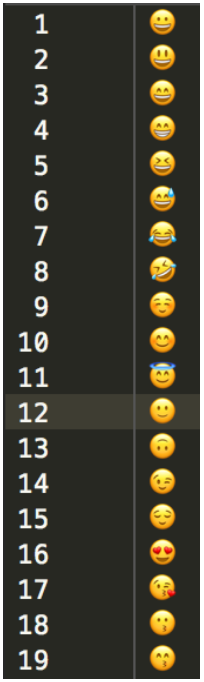
\includegraphics[scale=0.7]{emojiexample}
\centering
\caption{Example of emojis that we extract from tweets}
\label{fig:emojis}
\end{figure}

\subsection{Weather Data}
We access weather data for each location through the OpenWeatherMap API. We use PyOWM\footnote{https://github.com/csparpa/pyowm}, an open-source python wrapper, to simplify API calls. Weather data is collected concurrently with Twitter data. At the end of each 2 hour interval, we collect the current atmospheric condition in each city. Examples of atmospheric conditions include rain, snow, clear, etc. In the data we collected, there are 8 classes of conditions: clouds, clear, rain, drizzle, mist, fog, snow, haze, and dust.

\subsection{Preprocessing}
One issue that we encountered was that some of the emoji vectors were extremely sparse. In some cities, such as Nashville, almost every vector only had a few emojis. Therefore, we only include vectors in which the sum of its elements is greater than 40. For classification, each atmospheric condition is represented using a number from the range 0-7. In the case of binary classification, we consider clear to be a positive weather condition and represent it with a 0. We consider all other conditions to be negative and represent these using a 1. Our final data set consisted of 977 data pairs.

\section{Learning Algorithms}
We compare 5 learning algorithms on our classification tasks: ZeroR, a Gaussian Mixture Model (GMM), an Artificial Neural Network (ANN), a Decision Tree, and Naive Bayes. We use ZeroR to establish a baseline, and we use a GMM to evaluate how our data clusters. We implement all models, with the exception of the ANN, using Scikit-Learn\footnote{http://scikit-learn.org/stable/}.

Our ANN is implemented using Keras\footnote{https://keras.io/}. The model architecture can be seen in Figure \ref{fig:neuralnet}. We use a ReLU activation function, binary crossentropy to evaluate our loss, and adam as our optimizer\cite{Nair2010}\cite{Kingma2015}. The model is trained for 20 epochs.

\begin{figure}[h]
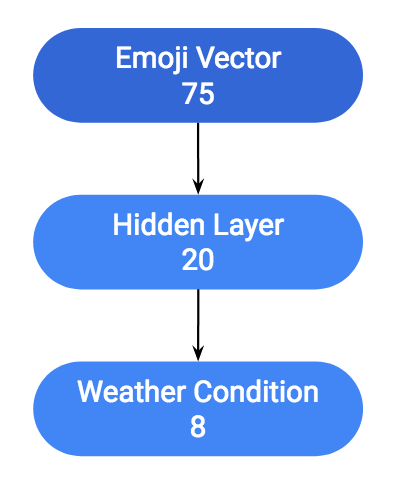
\includegraphics[scale=0.7]{neuralnet}
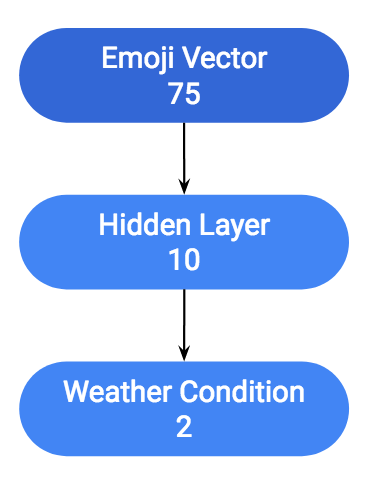
\includegraphics[scale=0.7]{neuralnetbinary}
\centering
\caption{Structure of our artificial neural networks. Left: ANN for standard classification. Right: ANN for binary classification. The numbers below the name of each layer represents the number of nodes in the layer.}
\label{fig:neuralnet}
\end{figure}

\section{Results}\label{results}
In this section we describe the results.

\section{Conclusions}\label{conclusions}
Conclusion goes here.

\newpage
\bibliographystyle{plain}
\bibliography{emoji}

\end{document}
